\chapter{Organizzazione fisica dei dati}
Un requisito fondamentale di un sistema di gestione di basi di dati è l'efficienza, cioè la capacità di rispondere alle richieste dell'utente il più rapidamente possibile. Poiché una particolare organizzazione fisica dei dati può rendere efficiente l'elaborazione di particolari richieste, bisogna tener presente quali operazioni saranno effettuate più frequentemente.

Generalmente ad ogni relazione corrisponde un file di record, dove ogni attributo corrisponde ad un campo e ogni tupla ad un record.

I file sono memorizzati su disco, ogni disco è partizionato in blocchi di formato fisso e ogni blocco corrisponde generalmente ad un settore di una traccia. Il costo di un accesso a disco, cioè del trasferimento di un blocco da o a memoria secondaria è molto superiore a quello di elaborazione di un blocco in memoria principale. Pertanto la valutazione del tempo di risposta del sistema ad una richiesta dell'utente viene effettuata in termini di numero di accessi a disco.

In realtà non sempre quando si deve elaborare un blocco è necessario effettuare un accesso
a disco, in quanto il sistema quando trasferisce un blocco in memoria principale lo
memorizza in un buffer e mantiene i blocchi trasferiti fin quando è possibile ricordando quali blocchi sono nei buffer. Inoltre il costo di un accesso a disco non è fisso, ma dipende dalla posizione del blocco rispetto all'ultimo blocco trasferito in quanto da ciò dipendono sia lo spostamento della testina da un cilindro all'altro sia la rotazione del disco. Tuttavia per valutare i costi delle operazioni elementari su file con determinata organizzazione fisica assumeremo che ogni lettura e scrittura di un blocco richieda il trasferimento del blocco da o a memoria secondaria e che ogni accesso a memoria secondaria abbia costo costante.

\section{Record}
Come abbiamo detto i record contengono campi che corrispondono agli attributi di relazione. Oltre a questi campi, però, un record può contenere campi che forniscono informazioni sul record stesso o che puntano ad altri record. Ad esempio alcuni byte possono essere utilizzati per specificare il tipo del record, la sua lunghezza o un bit di cancellazione oppure, se si vuole spostare il record all'interno del blocco, si può utilizzare una coppia $(b,k)$, dove $b$ è l'indirizzo del blocco che contiene il record e $k$ il valore di uno o più campi che servono come chiave.

Per poter accedere ad un campo di un record contenente un dato è necessario sapere qual'è il primo byte del campo nel record. Se tutti i campi del record hanno lunghezza fissa, basta ordinarli, infatti, una volta ordinati, l'inizio di ciascun campo sarà sempre ad un numero fisso di byte dall'inizio del record (\textit{offset del campo}). Se il record contiene campi a lunghezza variabile allora l'offset di un campo può variare da un record all'altro, in tal caso si possono usare due strategie: o all'inizio di ogni campo c'è un contatore che specifica la lunghezza del campo in numero
di byte, oppure all'inizio del record ci sono dei puntatori all'inizio di ciascun campo a lunghezza variabile.

\section{Blocchi}
Analogamente a quanto accade per un record, anche in un blocco può essere riservato spazio per memorizzare informazioni sul blocco stesso o per collegarlo ad altri blocchi in una lista.

Se un blocco contiene solo record di lunghezza fissa allora il blocco può essere suddiviso in aree (sotto-blocchi) di lunghezza fissa ciascuna delle quali può contenere un record. Se un blocco contiene record di lunghezza variabile per accedere ai record si possono usare due strategie: o si pone in ogni record un campo che ne specifica la lunghezza e, per calcolare il byte di inizio di un record, si somma all'offset del record precedente la sua lunghezza, oppure si pone all'inizio del blocco una directory contenente i puntatori ai record nel blocco. Poiché il numero di record che possono entrare in un blocco è in questo caso variabile, la directory può essere realizzata in uno dei modi seguenti: preceduta da un campo che specifica quanti sono i puntatori, come una lista di puntatori che termina con il valore 0 oppure di dimensione fissa con valore 0 negli spazi che non contengono puntatori.

\section{File}
In questo paragrafo esamineremo diversi tipi di organizzazione fisica di file che consentono la ricerca di record in base al valore di uno o più campi chiave. Il termine "chiave" non va inteso nel senso in cui viene usato nella teoria relazionale, in quanto un valore della chiave non necessariamente identifica univocamente un record nel file. 

Le operazioni elementari su questi tipi di file sono: \textit{ricerca}, \textit{inserimento}, \textit{cancellazione} e \textit{modifica}.

\subsection{File heap}
In questo tipo di organizzazione i record sono memorizzati nei blocchi senza alcun ordine: un record viene sempre inserito come ultimo record del file e l'accesso al file avviene attraverso una directory che contiene i puntatori ai blocchi (vedi Figura \ref{fig:file-heap}). 

\begin{figure}[h]
    \centering
    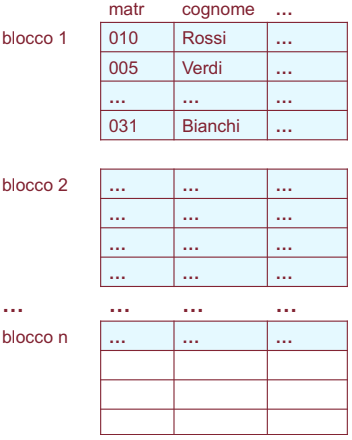
\includegraphics[width=0.35\linewidth]{images/file-heap.PNG}
    \caption{File heap}
    \label{fig:file-heap}
\end{figure}

Denotiamo con $b$ il numero di blocchi del file ed esprimiamo in termini di $b$ il costo delle varie operazioni:
\begin{itemize}
    \item Se la chiave di ricerca non identifica univocamente un record nel file, poiché non esiste alcun particolare ordinamento dei record, per effettuare una ricerca occorre scandire tutto il file sequenzialmente e, quindi, il costo di una ricerca è dato da $b$. 

    Se la chiave di ricerca identifica univocamente un record nel file, la ricerca di un record con un dato valore per la chiave richiede in media $b/2$ accessi. Infatti, per la ricerca di un record che si trova nell'i-esimo blocco sono necessari $i$ accessi (in lettura); pertanto se denotiamo con $N$ il numero di record nel file e con $R$ il numero di record che possono essere memorizzati in un blocco ($N/R=b$), il numero medio di accessi necessari per la ricerca di un record è data dalla somma per accedere ai singoli record diviso il numero di record:
    \begin{equation*}
        \frac{R*1+R*2+...+R*i+...+R*b}{N}=\frac{R(1+2+...+i+...+b)}{N}=\frac{R}{N}\frac{b(b+1)}{2}=\frac{1}{b}\frac{b(b+1)}{2}\approx \frac{b}{2}
    \end{equation*}
    \item L'inserimento di un record richiede la lettura dell'ultimo blocco del file; se in tale blocco c'è spazio sufficiente per memorizzare il nuovo record, il record viene inserito, altrimenti viene chiesto un nuovo blocco al file system. Dopo l'inserimento del record nel blocco, il blocco deve essere scritto su memoria secondaria. Quindi 2 accessi (uno per lettura e uno per scrittura) sono sufficienti per l'inserimento di un record. Se non ammettiamo duplicati l'inserimento deve essere preceduto dalla ricerca, quindi dobbiamo aggiungere una media di $b/2$ accessi per verificare che non esista già un record con la chiave data.
    \item La cancellazione di un record con un dato valore per la chiave richiede $b/2$ accessi in lettura per la ricerca e 1 accessi in scrittura.
    \item La modifica di un record con un dato valore per la chiave richiede $b/2$ accessi in lettura per la ricerca e 1 accessi in scrittura.
\end{itemize}

\begin{Example}{File heap}{}
    \textit{Dati $N=151$ record di 30 byte e dei blocchi di 65 byte che contengono dei puntatori al prossimo blocco (4 byte), calcolare il numero di blocchi necessari per memorizzare i record.}

    Calcoliamo il numero di record che entrano in ogni blocco:
    \begin{equation*}
        \frac{(65-4)}{30}=\frac{61}{30}=2.03=2\mbox{ record per blocco}
    \end{equation*}
    Troviamo ora il numero di blocchi che occorrono per memorizzare tutti i record:
    \begin{equation*}
        \frac{151}{2}=75.5=76\mbox{ blocchi}
    \end{equation*}
\end{Example}

\subsection{File hash}
In questo tipo di organizzazione i record sono ripartiti in bucket (secchi) in base al valore della chiave. Se $B$ è il numero dei bucket, questi vengono numerati da 0 a $B-1$. Dato un valore $v$ per la chiave il numero del bucket in cui deve trovarsi un record con chiave $v$ è calcolato mediante una funzione che prende il nome di \textit{funzione hash}. Una funzione hash per essere "buona" deve ripartire uniformemente i record nei bucket, cioè al variare del valore della chiave deve assumere con la stessa probabilità uno dei valori compresi tra 0 e $B-1$.

Ciascun bucket è costituito da uno o più blocchi ed è organizzato come un heap. L'accesso ai bucket avviene attraverso la bucket directory che contiene B elementi dove l'i-esimo elemento contiene l'indirizzo del primo blocco dell'i-esimo bucket. Tutti i blocchi di un bucket sono collegati tra loro mediante puntatori in una lista (vedi Figura \ref{fig:file-hash}).

\begin{figure}[h]
    \centering
    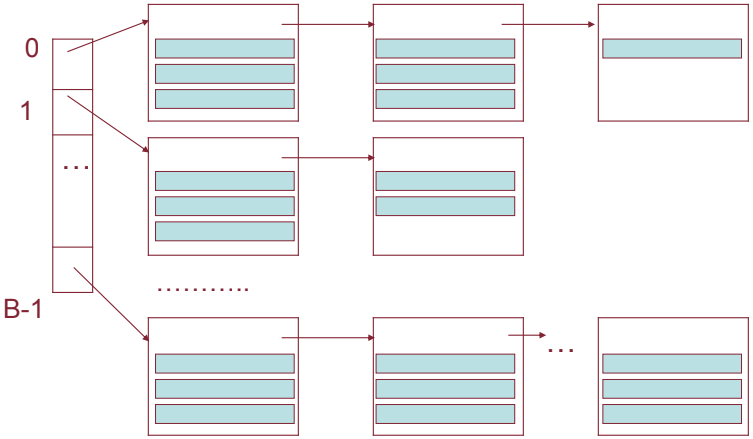
\includegraphics[width=0.6\linewidth]{images/file-hash.PNG}
    \caption{File hash}
    \label{fig:file-hash}
\end{figure}

Una qualsiasi operazione (ricerca, inserimento, cancellazione, modifica) su un file hash richiede la valutazione di $h(v)$ (dove $v$ è un valore per la chiave e $h$ è la funzione hash) per individuare il bucket in cui deve trovarsi il record con chiave $v$; successivamente, l'operazione viene effettuata sul bucket che, come già detto, è organizzato come un heap. Se la funzione hash distribuisce uniformemente i record nei bucket, ogni bucket è costituito da un numero di blocchi che è $1/B-esimo$ del numero di blocchi di cui è costituito l'intero file. Pertanto il costo richiesto per un'operazione è approssimativamente $1/B-esimo$ del costo che sarebbe richiesto per fare la stessa operazione se il file fosse organizzato come un heap. Si osservi che, poiché l'inserimento di un record viene effettuato sull'ultimo blocco del bucket, è opportuno che la bucket directory contenga anche, per ogni bucket, un puntatore all'ultimo record del bucket.

Da quanto detto appare evidente che quanti più sono i bucket tanto più basso è il costo di ogni operazione. D'altra parte limitazioni al numero dei bucket derivano dalle seguenti considerazioni: ogni bucket deve avere almeno un blocco; se le dimensioni della bucket directory sono tali che non può essere mantenuta in memoria principale durante l'utilizzo del file, ulteriori accessi sono necessari per leggere i blocchi della bucket directory.

\begin{Example}{File hash}{}
    \textit{Supponiamo di avere un file di 250.000 record, dove ogni record occupa 300 byte, di cui 75 per il campo chiave. Ogni blocco contiene 1024 byte, di cui un puntatore al blocco che occupa 4 byte. Rispondere alle seguenti domande: (a) se usiamo una organizzazione hash con 1200 bucket, quanti blocchi occorrono per la bucket directory? (b) quanti blocchi occorrono per i bucket, assumendo una distribuzione uniforme dei record nei bucket? (c) assumendo ancora che tutti i bucket contengano il numero medio di record, qual è il numero medio di accessi a blocco per ricercare un record che sia presente nel file? (d) Quanti bucket dovremmo creare per avere invece un numero medio di accessi a blocco inferiore o al massimo uguale a 10, assumendo comunque una distribuzione uniforme dei record nei bucket?}

    Indichiamo con $NR=250000$ il numero di record, $R=300$ i byte di un record, $K=75$ i byte del campo chiave, $CB=1024$ i byte di un blocco, $P=4$ i byte del puntatore.
    \begin{enumerate}[label=(\alph*)]
        \item Indichiamo con $B$ il numero di bucket e con $BD$ il numero di blocchi per la bucket directory. La bucket directory è essenzialmente un array di puntatori indicizzato da 0 a $B-1$.

        Vediamo prima quanti puntatori entrano in un blocco:
        \begin{equation*}
            RB=\frac{CB}{P}=\frac{1024}{4}=256
        \end{equation*}
        Ci occorreranno:
        \begin{equation*}
            BD=\frac{B}{RB}=\frac{1200}{256}=4.69=5
        \end{equation*}

        \item In un blocco dobbiamo quindi memorizzare il maggior numero possibile di record e in più un puntatore per un eventuale prossimo blocco nel bucket. Se indichiamo con $M$ il massimo numero di record memorizzabili in un blocco, avremo:
        \begin{equation*}
            M*R+P\leq CB\implies 300M+4\leq 1024\hspace{1cm}M\leq \frac{1020}{300}=3.4=3
        \end{equation*}
        Se la distribuzione dei record nei bucket è uniforme, indicando con $RB$ il numero di record in un bucket, avremo:
        \begin{equation*}
            RB=\frac{NR}{B}=\frac{250000}{1200}=208.3=209
        \end{equation*}
        Indicando con $NB$ il numero di blocchi per ogni bucket, occorrono quindi:
        \begin{equation*}
            NB=\frac{RB}{M}=\frac{209}{3}=70
        \end{equation*}
        Indicando con $BB$ il numero complessivo di blocchi per il file hash, avremo:
        \begin{equation*}
            BB=NB*B=70*1200=84000
        \end{equation*}

        \item In un bucket avremo come detto $NB = RB/M = 70$ blocchi per bucket. Poiché la ricerca avviene solo sul bucket individuato in base al risultato dell'applicazione della funzione hash alla chiave del record, avremo un numero di accessi a blocco pari a quello che si avrebbe su un heap della stessa dimensione del bucket (cioè $1/B$ rispetto alla dimensione originale). In media accederemo alla metà di questi blocchi, quindi indicando con $MA$ il numero medio di accessi, avremo:
        \begin{equation*}
            MA=\frac{NB}{2}=\frac{70}{2}=35
        \end{equation*}

        \item Per avere un numero di accessi a blocco inferiore o al massimo uguale a 10, riscriviamo l'espressione di MA in modo che vi compaia esplicitamente il numero di bucket $B$:
        \begin{equation*}
            MA=\frac{NB}{2}=\frac{\frac{RB}{M}}{2}=\frac{\frac{\frac{NR}{B}}{M}}{2}=\frac{NR}{2(B*M)}\leq10\hspace{1cm}B\geq\frac{NR}{20M}=\frac{250000}{20*3}=4167
        \end{equation*}
    \end{enumerate}
    Verifichiamo infatti che in questo caso avremo:
    \begin{equation*}
        RB=\frac{NB}{B}=\frac{250000}{4167}=60\hspace{1cm}NB=\frac{RB}{M}=20\hspace{1cm}MA=\frac{NB}{2}=10
    \end{equation*}
\end{Example}

\begin{Example}{File hash}{}
    \textit{Supponiamo di avere un file di 780.000 record, dove ogni record occupa 250. Ogni blocco contiene 1024 byte e un puntatore a blocco occupa 4 byte. Usiamo una organizzazione hash con 2500 bucket. (a) Quanti blocchi dobbiamo utilizzare complessivamente per la bucket directory e per i bucket, assumendo una distribuzione uniforme dei record nei bucket? (b) Quanti blocchi dobbiamo utilizzare complessivamente per i bucket, assumendo che il 30\% dei record sia distribuito in modo uniforme su 1000 bucket, e che il restante 70\% dei record sia distribuito in modo uniforme sui 1500 bucket rimanenti?}

    Definiamo con $NR=780000$ il numero di record, $R=250$ i byte del record, $P=4$ i byte del puntatore, $CB=1024$ i byte del blocco, $B=2500$ il numero di bucket.
    \begin{enumerate}[label=(\alph*)]
        \item Calcoliamo innanzitutto quanti puntatori entrano in ogni blocco della bucket directory:
        \begin{equation*}
            PC=\frac{CB}{P}=\frac{1024}{4}=256
        \end{equation*}
        Calcoliamo quindi quanti blocchi occorrono per la bucket directory, cioè per memorizzare 2500 puntatori:
        \begin{equation*}
            BD=\frac{B}{PB}=\frac{2500}{256}=9,7=10
        \end{equation*}
        Assumendo una distribuzione uniforme, dobbiamo prima di tutto calcolare quanti record devono essere memorizzati in ogni bucket:
        \begin{equation*}
            RB=\frac{NR}{B}=\frac{780000}{2500}=312
        \end{equation*}
        Vediamo ora quanti record possono essere memorizzati in un blocco, tenendo conto del fatto che ogni blocco di un bucket deve contenere anche un puntatore al blocco successivo:
        \begin{equation*}
            RBL=\frac{CB-P}{R}=\frac{1020}{250}=4.08=4
        \end{equation*}
        Calcoliamo infine quanti blocchi occorrono per ogni bucket:
        \begin{equation*}
            BB=\frac{RB}{RBL}=\frac{312}{4}=78
        \end{equation*}
        Complessivamente ci occorrono:
        \begin{equation*}
            BD + BB * B = 10 + 78 * 2500 = 195010
        \end{equation*}

        \item Il 30\% dei record è distribuito uniformemente su 1000 bucket, il rimanente 70\% dei record è distribuito uniformemente su 1500 bucket. Quindi il numero di record che va distribuito uniformemente su 1000 bucket è:
        \begin{equation*}
            N1000=\frac{780000*30}{100}=234000
        \end{equation*}
        Per ogni bucket dei 1000 avremo quindi:
        \begin{equation*}
            RB1000=\frac{N1000}{1000}=234
        \end{equation*}
        Quindi per ognuno di questi 1000 bucket occorrono:
        \begin{equation*}
            B1000=\frac{RB1000}{RBL}=\frac{234}{4}=58.5=59
        \end{equation*}
        Il numero di record che va distribuito uniformemente su 1500 bucket è:
        \begin{equation*}
            N1500=N-N1000=780000-234000=546000
        \end{equation*}
        Per ogni bucket dei 1500 avremo quindi:
        \begin{equation*}
            RB1500=\frac{N1500}{1500}=364
        \end{equation*}
        Quindi per ognuno di questi 1500 bucket occorrono quindi:
        \begin{equation*}
            B1500=\frac{RB1500}{RBL}=\frac{364}{4}=91
        \end{equation*}
        In totale avremo:
        \begin{equation*}
            B1000 * 1000 + B1500 * 1500 = 59 * 1000 + 91 * 1500 = 195.500
        \end{equation*}
    \end{enumerate}
\end{Example}

\subsection{File con indice (ISAM)}
Nella presentazione di questo tipo di organizzazione, spesso chiamato ISAM (\textit{Indexed Sequential Access Method}), assumeremo che il valore della chiave identifica univocamente un record del file e, inizialmente, assumeremo che i record non siano puntati. 

Inizialmente il file principale viene ordinato in base al valore crescente della chiave e viene memorizzato lasciando in ogni blocco una certa percentuale (ad esempio il 20\%) di spazio non utilizzato per l'inserimento di nuovi record. Quindi viene creato un nuovo file indice che contiene un record per ogni blocco del file principale e formato da due campi che contengono: un puntatore ad un blocco dal file principale e il più piccolo valore della chiave presente nel blocco (vedi Figura \ref{fig:file-indice}). L'unica eccezione è rappresentata dal primo blocco per il quale viene preso anziché il valore della chiave del primo record, un valore (denotato con $-\infty$) che è più piccolo di qualsiasi valore che può essere assunto dalla chiave.

\begin{figure}[h]
    \centering
    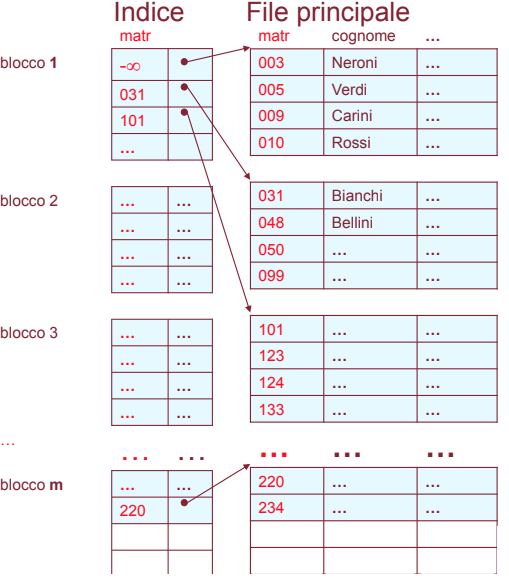
\includegraphics[width=0.5\linewidth]{images/file-indice.PNG}
    \caption{File con indice}
    \label{fig:file-indice}
\end{figure}

Identifichiamo ora il costo delle varie operazioni su questa struttura:
\begin{itemize}
    \item I record del file indice possono a loro volta essere ordinati in base al valore della chiave, in questo modo è possibile utilizzare la \textit{ricerca binaria}. Siano $B_1, B_2,..., B_m$ i blocchi del file indice; si comincia con il considerare il blocco $B_{[m/2]}$ e si confronta il valore w della chiave nel primo record di tale blocco con $v$; se $v=w$ la ricerca ha termine; se $v<w$ si ripete il procedimento come se il file indice fosse costituito dai blocchi $B_1, B_2,..., B_{[m/2-1]}$; se invece $v>w$ si ripete il procedimento come se il file indice fosse costituito dai blocchi $B_{[m/2]}, B_{[m/2+1]},..., B_m$. Il procedimento viene iterato fino a quando ci si riduce a considerare un unico blocco; a questo punto si scandisce il blocco per trovare un valore della chiave che ricopre $v$. Poiché ad ogni passo il numero di blocchi su cui deve essere effettuata la ricerca viene dimezzato, dopo al più $\log_2(m)$ passi la ricerca è ristretta ad un unico blocco.
    
    Un altro metodo è costituito dalla \textit{ricerca per interpolazione}. Questo tipo di ricerca è basato sulla conoscenza della distribuzione dei valori della chiave. In altre parole per poter effettuare questa ricerca si deve disporre di una funzione $f$ che dati tre valori $v_1, v_2, v_3$ della chiave fornisce un valore che è la frazione dell'intervallo di valori della chiave compresi tra $v_2$ e $v_3$ in cui deve trovarsi $v_1$. In tal caso, se $B_1, B_2,..., B_m$ sono i blocchi del file indice (o di una sua parte) e $v_2$ è il valore della chiave nel primo record di $B_1$ e $v_3$ è il valore della chiave nell'ultimo record di $B_m$ allora $v_1$ deve essere confrontato con il valore della chiave nel primo record di $Bi$ , dove $i=f(v_1,v_2,v_3)*m$; analogamente a quanto accade nella ricerca binaria, se $v_1$ è minore di tale valore allora il procedimento deve essere ripetuto sui blocchi $B_1, B_2,..., B_{i-1}$ , mentre se è maggiore il procedimento deve essere ripetuto sui blocchi $B_i, B_{i+1},..., B_m$, finché la ricerca si restringe ad un unico blocco. E' stato mostrato che la ricerca per interpolazione richiede circa $1+log_2log_2(m)$ accessi.

    \item Per inserire un nuovo record nel file principale occorre innanzitutto ricercare il blocco $B_i$ del file principale in cui il record deve trovarsi in base al valore della chiave. Se in $B_i$ c'è spazio sufficiente, il record viene inserito in modo da rispettare l'ordinamento (quindi spostando eventualmente record con chiave maggiore). Altrimenti si possono seguire diverse strategie. Ad esempio si può verificare se c'è spazio sufficiente nel blocco successivo $B_{i+1}$; in tal caso, o il nuovo record o un record che era precedentemente in $B_i$ diventa il primo record di $B_{i+1}$ e, pertanto, il record del file indice che contiene il puntatore a $B_{i+1}$ deve essere modificato. Se $B_{i+1}$ non esiste ($B_i$ è l'ultimo blocco del file) oppure è pieno si può prendere in considerazione il blocco $B_{i-1}$ ed eventualmente procedere in modo simile ripartendo i record di tra $B_{i-1}$ e $B_i$; anche in questo caso sarà necessario apportare una modifica al file indice. Se anche $B_{i-1}$ è pieno oppure se $B_{i-1}$ non esiste ($B_i$ è il primo blocco del file), è necessario richiedere al sistema un nuovo blocco che seguirà $B_i$ e ripartire i record di $B_i$ tra $B_i$ e il nuovo blocco; quindi occorre inserire nel file indice il record relativo al nuovo blocco.

    \item Per cancellare un record dal file principale occorre innanzitutto ricercare il record, quindi cancellarlo, spostare i record nel blocco in modo da recuperare lo spazio lasciato libero. Se il record cancellato è il primo record del blocco occorre modificare nel file indice il record relativo al blocco. Se il record cancellato era l'unico record del blocco, il blocco viene restituito al sistema e nel file indice occorre cancellare il record relativo al blocco.

    \item Per modificare un record del file principale occorre innanzitutto ricercare il record; quindi, se la modifica non coinvolge campi della chiave, il record viene modificato e il blocco riscritto. Altrimenti la modifica equivale ad una cancellazione seguita da un inserimento.
\end{itemize}

Consideriamo ora il caso in cui il file principale contiene record puntati.

In tal caso la fase di inizializzazione non differisce dal caso precedente salvo che è preferibile lasciare più spazio libero nei blocchi per successivi inserimenti (vedi Figura \ref{fig:file-indice-puntato}). Infatti, poiché i record sono puntati, non possono essere spostati per mantenere l'ordinamento. Le operazioni saranno:
\begin{itemize}
    \item La ricerca di un record con chiave $v$ richiede la ricerca sul file indice di un valore della chiave che ricopre $v$ e quindi la scansione del bucket corrispondente.

    \item La cancellazione di un record richiede la ricerca del record e quindi la modifica dei bit di cancellazione nell'intestazione del blocco.

    \item La modifica di un record richiede la ricerca del record; quindi, se la modifica non coinvolge campi della chiave, il record viene modificato e il blocco riscritto. Altrimenti la modifica equivale ad una cancellazione seguita da un inserimento. In quest'ultimo caso non è sufficiente modificare il bit di cancellazione del record cancellato, ma è necessario inserire in esso un puntatore al nuovo record inserito in modo che questo sia raggiungibile da qualsiasi record che contenga un puntatore al record cancellato.
\end{itemize}

\begin{figure}[h]
    \centering
    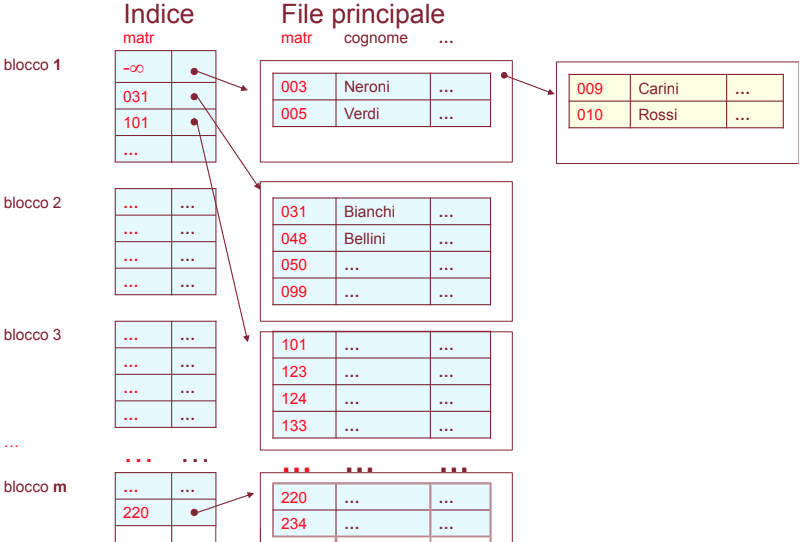
\includegraphics[width=0.7\linewidth]{images/file-indice-puntato.PNG}
    \caption{File con indice con record puntati}
    \label{fig:file-indice-puntato}
\end{figure}

Poiché non è possibile mantenere il file principale ordinato, se si vuole avere la possibilità di esaminare il file seguendo l'ordinamento della chiave occorre inserire in ogni record un puntatore al record successivo nell'ordinamento.

\begin{Example}{File con indice}{}
    \textit{Supponiamo di avere un file di 150.000 record. Ogni record occupa 250 byte, di cui 50 per il campo chiave. Ogni blocco contiene 1024 byte. Un puntatore a blocco occupa 4 byte.}

    \textit{(a)Se usiamo un indice ISAM sparso, e assumiamo che i record non siano puntati e che il fattore di utilizzo dei blocchi del file principale sia 0,7 (cioè i blocchi non sono completamente pieni, ma pieni al più al 70\%), quanti blocchi dobbiamo utilizzare per l'indice? (b) Se usiamo un indice ISAM sparso, e assumiamo che i record siano puntati e che i blocchi del file principale siano pieni, quanti blocchi dobbiamo utilizzare per l'indice? (c) Se utilizziamo la ricerca binaria, quale è il numero massimo di accessi a blocco per ricercare un record presente nel file nei casi (a) e (b), supponendo nel caso (b) di non avere liste di overflow?}

    \begin{enumerate}[label=(\alph*)]
        \item I record sono di taglia fissa, quindi non occorrono puntatori all'inizio del blocco; poiché i record non sono puntati, nei blocchi del file principale non occorre un puntatore al prossimo blocco. L'esercizio fornisce il fattore di occupazione attuale dei blocchi del file del file principale, ma non indica un fattore di occupazione per i blocchi indice, quindi possiamo assumere che siano pieni.

        Dobbiamo stabilire quanti record indice occorrono, quindi sapendo che l'indice contiene un record per ogni blocco del file principale, dobbiamo calcolare quanti sono questi blocchi. Sappiamo che i blocchi dati sono occupati al più al 70\% (indichiamo questa quantità con PO), quindi prima di tutto vediamo quanti record interi possono essere contenuti al massimo nella porzione indicata di blocco. Indicando con M questo numero, avremo che:
        \begin{equation*}
            M=\frac{(CB*PO)}{R}=\frac{(1024*\frac{70}{100})}{250}=2.86\approx 2
        \end{equation*}
        Il numero di blocchi da indicizzare, indicato con BF, sarà quindi:
        \begin{equation*}
            BF=\frac{NR}{M}=\frac{150000}{2}=75000
        \end{equation*}
        Ogni record indice è composto da chiave e puntatore al blocco, quindi occupa $RI = K + P$ byte, cioè RI = 54 byte. Dobbiamo ora calcolare quanti record indice interi possono essere contenuti in un blocco pieno, indicando con MI questo numero avremo:
        \begin{equation*}
            MI=\frac{CB}{RI}=\frac{1024}{54}=18
        \end{equation*}
        In definitiva, indicando con BI il numero di blocchi indice, avremo:
        \begin{equation*}
            BI=\frac{BF}{MI}=\frac{75000}{18}=4167
        \end{equation*}

        \item L'esercizio ci dice in questo caso che i blocchi dati sono pieni, e lo stesso possiamo assumere per i blocchi indice. Ogni blocco del file principale deve essere visto come parte di un bucket, e quindi dobbiamo anche prevedere spazio per un puntatore. Vediamo prima di tutto in queste nuove condizioni quanti record interi di dati entrano al massimo in un blocco:
        \begin{equation*}
            M=\frac{(CP-P)}{R}=\frac{1020}{250}=4.08\approx 4
        \end{equation*}
        Vediamo allora quanti blocchi vanno indicizzati indicando questo numero con BF avremo:
        \begin{equation*}
            BF=\frac{NR}{M}=\frac{150000}{4}=37500
        \end{equation*}
        A questo punto calcoliamo il numero di blocchi indice. La struttura dl blocco indice è identica a quella del caso precedente, quindi ricordiamo che la taglia del record indice è RI = 54 byte , che il numero massimo di record indice per blocco è MI = 18 e quindi occorrono:
        \begin{equation*}
            BI=\frac{BF}{MI}=\frac{37500}{18}=2084
        \end{equation*}

        \item In entrambi i casi la ricerca si effettua prima di tutto sui blocchi indice; assumiamo una ricerca binaria; i due casi si differenziano, perché nel caso di record non puntati dobbiamo ancora leggere in memoria un solo blocco di record di dati, mentre nel caso di record puntati l'indice punta ad un bucket che potrebbe contenere più blocchi di overflow, che vanno tutti esaminati. Nel nostro caso però l'esercizio dice esplicitamente che non ci sono liste di overflow, quindi in entrambe le configurazioni dobbiamo aggiungere un solo accesso a blocco, quindi nella configurazione (a) e (b) avremo rispettivamente:
        \begin{gather*}
            A = log_2 BI + 1 = log_2 4167 + 1 = 14\\
            A = log_2 BI + 1 = log_2 2084 + 1 = 13
        \end{gather*}
    \end{enumerate}
\end{Example}

\subsection{File B-tree}
Questa organizzazione è una generalizzazione del file con indice, infatti in un B-tree si accede al file attraverso
una gerarchia di indici. L'indice a livello più alto nella gerarchia è costituito da un unico blocco e quindi può risiedere in memoria principale durante l'utilizzo del file. 

Ogni blocco di un file indice è costituito di record contenenti una coppia $(v,b)$ dove $v$ è il valore della chiave del primo record della porzione del file principale che è accessibile attraverso il puntatore $b$; $b$ può essere un puntatore ad un blocco del file indice a livello immediatamente più basso oppure (nei record del file indice nel più basso livello della gerarchia) ad un blocco del file principale. I blocchi degli indici e del file principale devono essere sempre pieni almeno per metà (vedi Figura \ref{fig:file-btree}).

\begin{figure}[h]
    \centering
    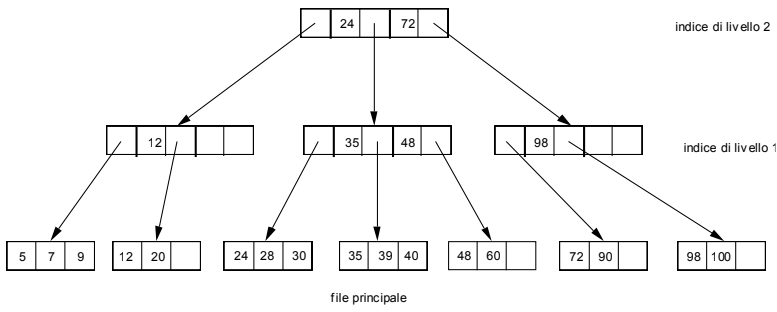
\includegraphics[width=0.7\linewidth]{images/file-btree.PNG}
    \caption{File B-tree}
    \label{fig:file-btree}
\end{figure}

\begin{itemize}
    \item Durante la ricerca di un record con un dato valore per la chiave si accede agli indici a partire da quello a livello più alto; a mano a mano che si scende nella gerarchia di indici si restringe la porzione (insieme di blocchi) del file principale in cui deve trovarsi il record desiderato, fino a che, nell'ultimo livello (il più basso nella gerarchia) tale porzione è ristretta ad un unico blocco. 

    Più in dettaglio, per ricercare il record del file principale con un dato valore $v$ per la chiave si procede nel modo seguente. Si parte dall'indice a livello più alto (che è costituito da un unico blocco) e ad ogni passo si esamina un unico blocco. Se il blocco esaminato è un blocco del file principale, tale blocco è quello in cui deve trovarsi il record desiderato; se, invece, è un blocco di un file indice, si cerca su tale blocco un valore della chiave che ricopre $v$ e si segue il puntatore associato (che sarà o un puntatore ad un blocco dell'indice al livello immediatamente inferiore o un blocco del file principale). Per valutare il costo di un'operazione di ricerca, assumiamo, per comodità, che il numero di record del file principale che possono essere memorizzati in un blocco sia un numero dispari $2e-1$, che il numero di record di un file indice che possono essere memorizzati in un blocco sia un numero dispari $2d-1$ (cioè, poiché ogni blocco è pieno almeno per metà, ogni blocco del file principale contiene almeno $e$ record e ogni blocco di un indice contiene almeno $d$ record). Con tali assunzioni il file principale ha al più $n/e$ blocchi, dove $n$ è il numero di record del file principale. Poiché ad ogni blocco del file principale corrisponde un record nel file indice al livello 1 (il più basso nella gerarchia) il numero di record del file indice a livello più basso sarà $n/e$ e, per l'ipotesi fatta (ogni blocco è pieno almeno per metà), questi $n/e$ record saranno memorizzati in al più $n/(ed)$ blocchi. Ripetendo tale ragionamento, si ottiene che l'indice a livello i ha $n/(ed^{i-1})$ record memorizzati in al più $n/(ed^i)$ blocchi. Sia $k$ il livello più alto della gerarchia; l'indice a livello $k$ avrà $n/(ed^{k-1})$ record memorizzati in al più $n/(ed^k)$ blocchi; poiché tale indice è costituito da un unico blocco $n/(ed^k)\geq1$. Poiché per ricercare un record del file principale si deve accedere ad un blocco per ogni livello di indice più al blocco del file principale che contiene il record desiderato, il numero di accessi necessari per un operazione di ricerca è $k+1\leq\log_d(n/e)+1$.

    \item Il numero di accessi necessari per effettuare l'inserimento del record con valore $v$ della chiave è dato dal numero di accessi necessari per ricercare il blocco in cui deve essere inserito il record con chiave $v$ più uno per riscrivere il blocco, se nel blocco c'è spazio sufficiente per inserire il record. Se, viceversa, nel blocco non c'è spazio sufficiente per inserire il nuovo record, l'operazione di inserimento può richiedere un numero ulteriore di accessi a causa della necessità di mantenere i blocchi pieni al meno per metà.

    \item Il numero di accessi necessari per effettuare la cancellazione del record con valore $v$ della chiave è dato dal numero di accessi necessari per ricercare il blocco in cui si trova il record con chiave $v$ più uno per riscrivere il blocco, se il blocco rimane pieno almeno per metà successivamente alla cancellazione. Se, viceversa, il blocco non rimane pieno almeno per metà successivamente alla cancellazione, l'operazione può richiedere un numero ulteriore di accessi.

    \item Il numero di accessi necessari per effettuare la modifica del record con valore $v$ della chiave è dato dal numero di accessi necessari per ricercare il blocco in cui si trova il record con chiave $v$ più uno per riscrivere il blocco, se la modifica non coinvolge campi della chiave, altrimenti è dato dalla somma degli accessi necessari per la cancellazione del record con chiave $v$ e quelli necessari per l'inserimento del record con il nuovo valore della chiave.
\end{itemize}

Notiamo che se il numero di record massimo che possiamo memorizzare è dispari, quindi esprimibile nella forma $2E-1$, possiamo direttamente considerare $E$ come occupazione  minima. Se il numero massimo di record che possiamo memorizzare è pari, quindi esprimibile come $2E$, possiamo considerare $E+1$ come occupazione minima.

\begin{Example}{File B-tree}{}
    \textit{Supponiamo di avere un file di 170.000 record dove ogni record occupa 200 byte, di cui 20 per il campo chiave. Ogni blocco contiene 1024 byte e un puntatore a blocco occupa 4 byte. Se usiamo un B-tree e assumiamo che sia i blocchi indice che i blocchi del file sono pieni al minimo, quanti blocchi vengono usati per il livello foglia (file principale) e quanti per l’indice, considerando tutti i livelli non foglia? Qual'è il costo di una ricerca in questo caso?}

    Per quanto riguarda i blocchi di dati nel livello foglia (file principale) indichiamo il numero massimo di record memorizzabili con MR, avremo:
    \begin{equation*}
        MR=\frac{CB}{R}=\frac{1024}{200}=5
    \end{equation*}
    Poiché il numero in questo caso è dispari ($MR = 2E-1 = 5$) per definizione, un blocco dati non conterrà mai meno di $E = 3$ record. A questo punto possiamo calcolare il numero di blocchi nel livello foglia, che sarà:
    \begin{equation*}
        BF=\frac{NR}{E}=\frac{170000}{3}=56667
    \end{equation*}
    A questo punto dobbiamo calcolare la capacità dei blocchi indice. Nei livelli indice del B-tree, ogni record, eccetto il primo, contiene una coppia (chiave, puntatore); il primo record invece contiene solo un puntatore (relativo al blocco dati che contiene i record con chiave minore della chiave contenuta nel record indice successivo). Indicando con MaxI tale numero dovremo avere:
    \begin{align*}
        (MaxI-1)*K+(MaxI)*P\leq CB\iff (MaxI-1)*20+(MaxI)*4\leq1024\iff\\MaxI\leq\frac{1044}{24}=43.5\approx43
    \end{align*}
    Volendo il minimo numero di blocchi abbiamo $2D-1=MaxI\iff 2*D-1=43\iff D=22$. Verifichiamo però che la metà dei record riempia la metà del blocco, considerando che il primo è solo puntatore: $21*(20+4)+4=508$ che è meno della metà del blocco  quindi per l’occupazione minima aggiungiamo 1 record (arriviamo a occupare 532). Quindi l'occupazione minima sarà $MinI=23$ record indice per blocco indice.

    Al primo livello di indice avremo quindi $B1=\frac{BF}{MinI}=\frac{56667}{23}=2463.78=2464$ blocchi indice. Ad ognuno di questi corrisponderà un record al secondo livello di indice, quindi $B2=\frac{B1}{MinI}=\frac{2464}{23}=107.13=108$ blocchi indice. Iterando il ragionamento avremo $B3=\frac{B2}{MinI}=\frac{108}{23}=5$ blocchi indice. A questo punto attenzione: anche questi ultimi sono blocchi a cui devono corrispondere dei record indice al livello superiore. Arriviamo così alla radice, che deve contenere sempre un unico blocco, e per la quale si rilascia il vincolo che sia piena almeno per metà (infatti nel nostro caso conterrà solo 5 record). Abbiamo allora $B4 = 1$ blocco indice.

    In conclusione abbiamo $BF = 56.667$ blocchi dati al livello foglia, e complessivamente $BI = B1 + B2 + B3 + B4 = 2464 + 108 + 5 + 1 = 2578$ blocchi nei 4 livelli di indice.

    Il costo di una ricerca sarà di 5 accessi (un blocco per ognuno dei 4 livelli di indice + 1 blocco del il file principale).
\end{Example}